\documentclass[border=10pt]{standalone}
\usepackage{amsfonts,amsmath,amssymb,amsthm}
\usepackage{tikz}
\usetikzlibrary{arrows.meta,shapes, calc}
\tikzset{%
  >={Latex[width=2mm,length=2mm]},
  % Specifications for style of nodes:
     base/.style = {rectangle, rounded corners, draw=black,
                           minimum width=4cm, minimum height=1.5cm,
                           text centered, font=\sffamily},
    stressUpdate/.style = {base, minimum width=2.5cm, fill=orange!15},
    newtonIteration/.style = {base, fill=blue!20},
    constitutiveModel/.style = {base, minimum width=2.5cm, fill=green!15},
    convergenceCheck/.style={newtonIteration, diamond, aspect=2},
}

\begin{document}    
  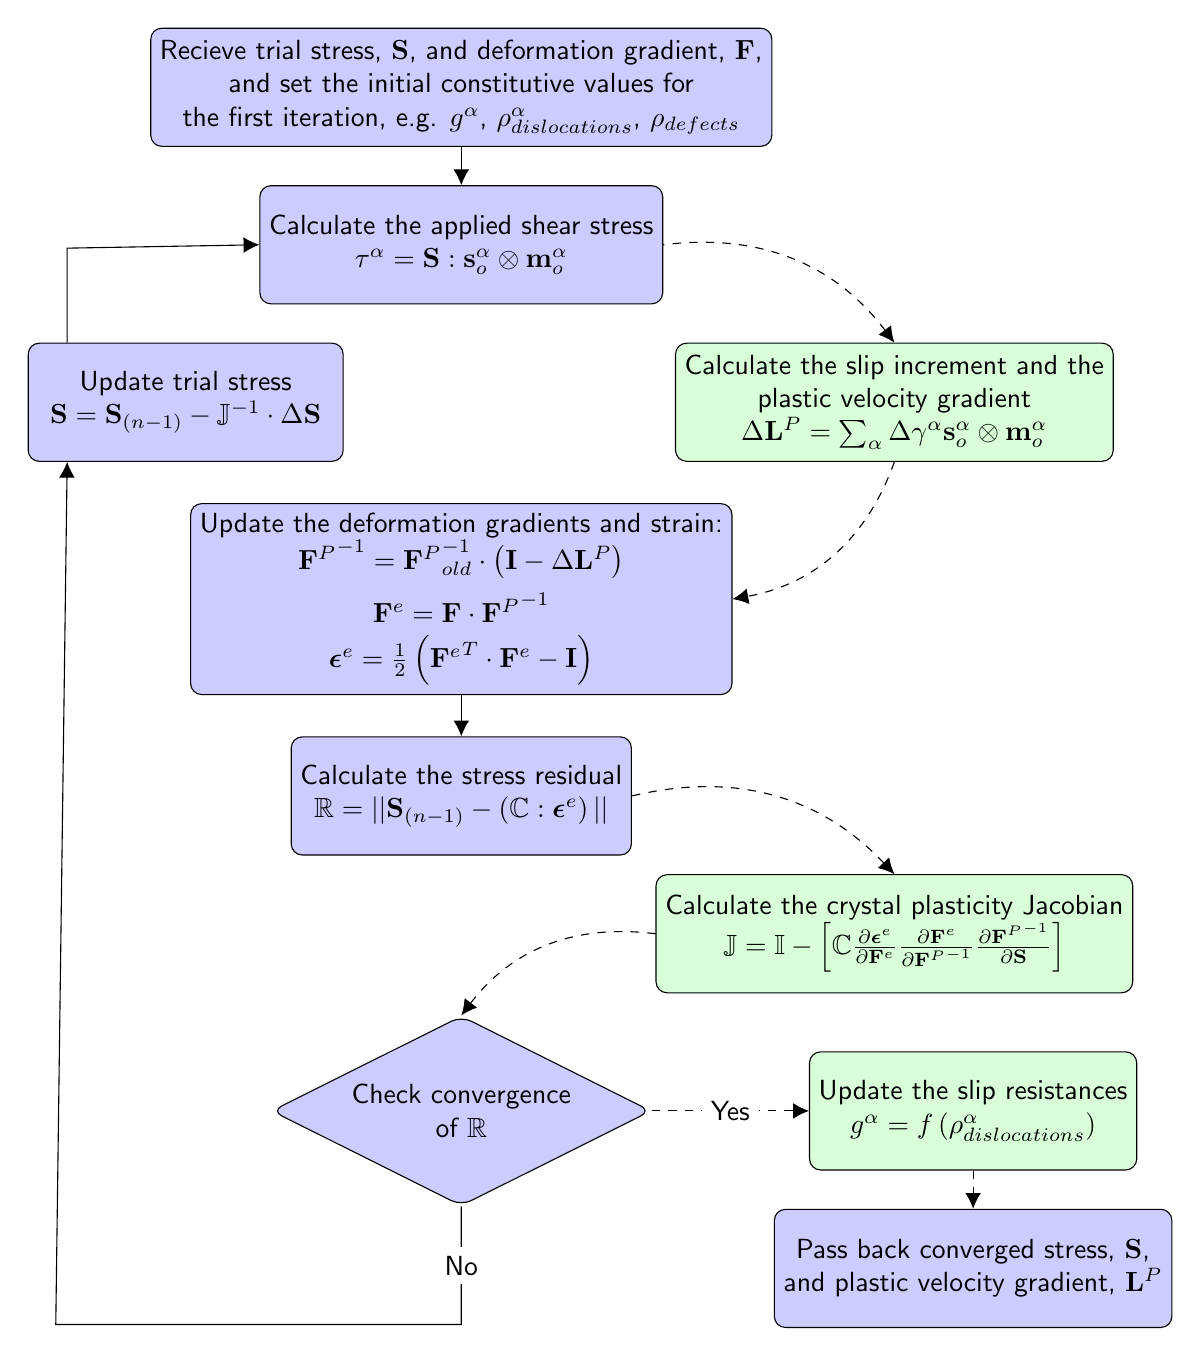
\begin{tikzpicture}[node distance=1.5cm,
    every node/.style={fill=white, font=\sffamily}, align=center]
  % Specification of nodes (position, etc.)
  \node (start)               [newtonIteration]
                              {Recieve trial stress, $\mathbf{S}$, and deformation gradient, $\mathbf{F}$,\\
                               and set the initial constitutive values for\\
                               the first iteration, e.g. $g^{\alpha}$, $\rho^{\alpha}_{dislocations}$, $\rho_{defects}$};
                               
  \node (calcTau)          [newtonIteration, below of=start, yshift=-0.5cm]
                              {Calculate the applied shear stress\\
                                $\tau^{\alpha} = \mathbf{S} : \mathbf{s}_o^{\alpha} \otimes \mathbf{m}_o^{\alpha}$};                              
                              
  \node (calcSlip)  [constitutiveModel, right of=calcTau, xshift=4.0cm, yshift=-2cm]
                              {Calculate the slip increment and the \\
                               plastic velocity gradient\\
                               $\Delta \mathbf{L}^P = \sum_{\alpha} \Delta \gamma^{\alpha} \mathbf{s}_o^{\alpha} \otimes \mathbf{m}_o^{\alpha}$}; 
  \node (updateDeformGrads)   [newtonIteration, below of=calcTau, yshift=-3cm]
                              {Update the deformation gradients and strain: \\
                               ${\mathbf{F}^P}^{-1} = {\mathbf{F}^P}^{-1}_{old} \cdot \left( \mathbf{I} - \Delta \mathbf{L}^P \right) $\\ [0.15cm]
                               $\mathbf{F}^e = \mathbf{F} \cdot {\mathbf{F}^P}^{-1}$ \\ [0.15cm]
                               $\boldsymbol{\epsilon}^e = \frac{1}{2} \left( {\mathbf{F}^e}^T \cdot \mathbf{F}^e - \mathbf{I} \right)$ };                            

  \node (updateResidual)    [newtonIteration, below of=updateDeformGrads, yshift=-1cm] 
                              {Calculate the stress residual\\
                              $\mathbb{R} = || \mathbf{S}_{(n-1)} - \left( \mathbb{C}: \boldsymbol{\epsilon}^e \right) ||$};
                              
  \node (calcJacobian)    [constitutiveModel, right of=updateResidual, xshift=4cm, yshift=-1.75cm]
                              {Calculate the crystal plasticity Jacobian\\
                              $\mathbb{J} = \mathbb{I} - \left[ \mathbb{C} \frac{\partial \boldsymbol{\epsilon}^e}{\partial \mathbf{F}^e}  \frac{\partial \mathbf{F}^e}{\partial {\mathbf{F}^P}^{-1}} \frac{\partial {\mathbf{F}^P}^{-1}}{\partial \mathbf{S}} \right]$};                          
                               
  \node (convergenceBlock)  [convergenceCheck, below of=updateResidual,  yshift=-2.5cm]
                             {Check convergence \\ 
                             of $\mathbb{R}$};
                             
  \node (updateResistances)  [constitutiveModel, right of=convergenceBlock, xshift=5cm]
                              {Update the slip resistances\\
                               $g^{\alpha} = f \left( \rho^{\alpha}_{dislocations} \right)$};                          
  
                              
  \node (updateStress)  [newtonIteration, left of=calcTau, xshift=-2cm, yshift=-2cm]
                              {Update trial stress\\
                               $\mathbf{S} = \mathbf{S}_{(n-1)} - \mathbb{J}^{-1} \cdot \Delta \mathbf{S}$};

 \node (passBackBlock) [newtonIteration, below of=updateResistances, yshift=-0.5cm] 
                             {Pass back converged stress, $\mathbf{S}$,\\
                        and plastic velocity gradient, $\mathbf{L}^P$};


 
  % Specification of lines between nodes specified above
  % with aditional nodes for description 
  \draw[->]  (start) to (calcTau);

  \draw[<-, bend right=30, dashed] (calcSlip.north) to (calcTau.east);
  \draw[->, bend left=30, dashed]  (calcSlip.south) to (updateDeformGrads.east);
  
  \draw[->]  (updateDeformGrads) to (updateResidual);

  \draw[<-, bend right=30, dashed] (calcJacobian.north) to (updateResidual.east);
  \draw[->, bend right=30, dashed]  (calcJacobian.west) to (convergenceBlock.north);
  
  \draw[->, dashed] (convergenceBlock.east) to node {Yes} (updateResistances.west);
  \draw[->, dashed]  (updateResistances.south) to (passBackBlock.north);
  
  \draw[->] (convergenceBlock.south) -- node{No} ++(0,-1.5) -- ++(-5.15,0) -- ($(updateStress.south west)!0.25!(updateStress.south)$);
  
  \draw[->,] ($(updateStress.north west)!0.25!(updateStress.north)$) -- ++(0,1.2) -- (calcTau.west);
 

  \end{tikzpicture}


\end{document}